\documentclass[twoside]{article}
\usepackage[UTF8]{ctex}
\usepackage{CJKutf8}
\usepackage{color}
\usepackage{natbib}
\usepackage{graphicx}
\usepackage{subfigure}
\usepackage{geometry}
\usepackage{amsmath}
\usepackage{mathrsfs}
\usepackage{algorithm}  
\usepackage{algorithmicx}  
\usepackage{algpseudocode}
\usepackage[backref]{hyperref}
\hypersetup{hidelinks}
\renewcommand{\algorithmicrequire}{\textbf{Input:}}  % Use Input in the format of Algorithm  
\renewcommand{\algorithmicensure}{\textbf{Output:}}
\geometry{a4paper, scale=0.8}

\title{\textbf{EE447 Homework}}
\author{付昊源 517021910753}
\date{March 29, 2020}

\begin{document}

\maketitle

%%%%%%%%%%%%%%%%%%%%%%%%%%%%%%
\section*{Problem Statement}
Suggest there are node $A$ and $B$ in this space, between which exists $n$ linked edges. The existing probability of the $i^{th}$ edge is $p_i$ where $i=1,2,\cdots n$. And the cost of detecting whether the $i^{th}$ edge exists is $c_i$. The graph is denoted as $G_n$, shown in Figure \ref{HW1_fig}. In this problem, we need to design a strategy to make sure the total cost for detecting is optimal in expectation, and prove its optimization.
\begin{figure}[h]
    \centering
    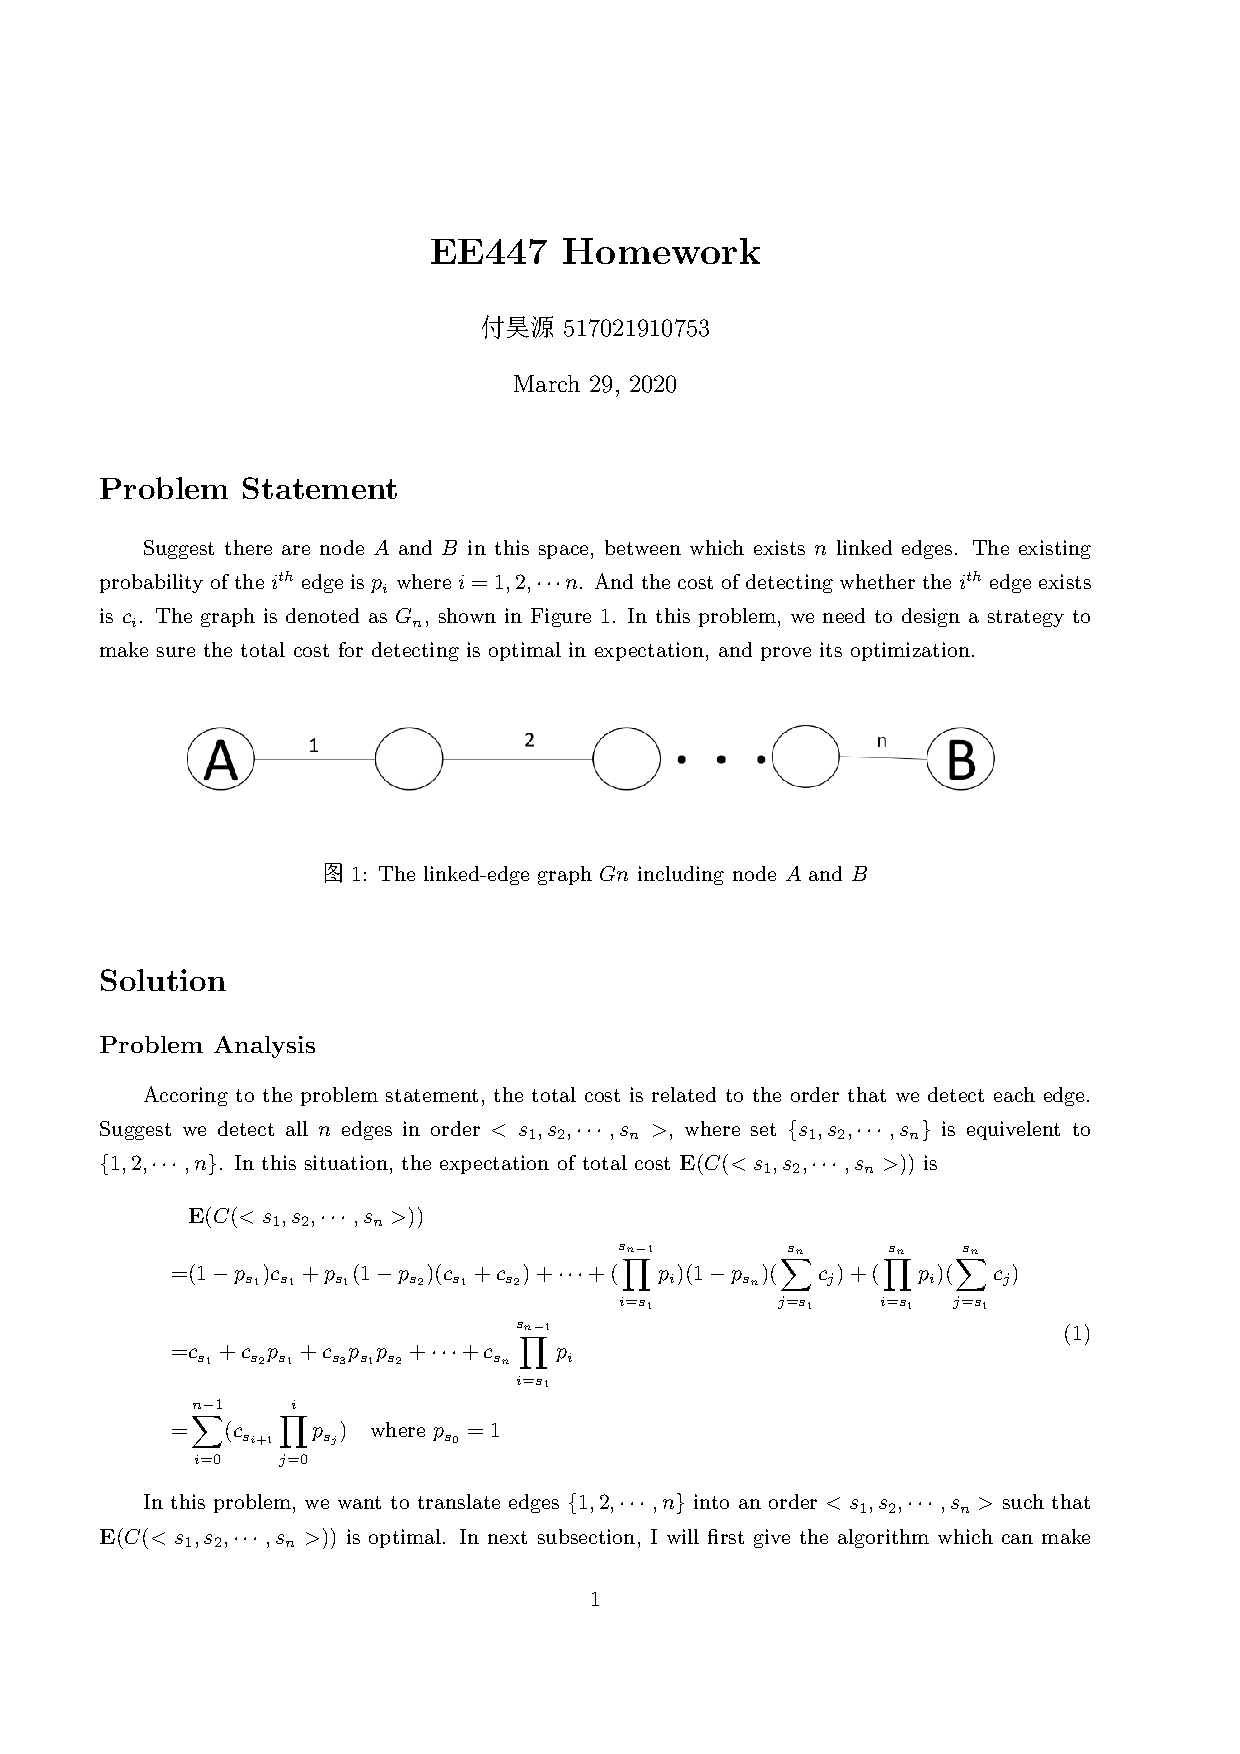
\includegraphics[width=0.9\linewidth]{HW1.PNG}
    \caption{The linked-edge graph $Gn$ including node $A$ and $B$}
    \label{HW1_fig}
\end{figure}

\section*{Solution}
\subsection*{Problem Analysis}
Accoring to the problem statement, the total cost is related to the order that we detect each edge. Suggest we detect all $n$ edges in order $<s_1,s_2,\cdots,s_n>$, where set $\{s_1, s_2,\cdots,s_n\}$ is equivelent to $\{1,2,\cdots,n\}$. In this situation, the expectation of total cost $\textbf{E}(C(<s_1,s_2,\cdots,s_n>))$ is
\begin{equation}\label{equation}
    \begin{aligned}
        &\textbf{E}(C(<s_1,s_2,\cdots,s_n>)) \\
        =& (1-p_{s_1})c_{s_1}+p_{s_1}(1-p_{s_2})(c_{s_1}+c_{s_2})+\cdots+(\prod_{i=s_1}^{s_{n-1}}p_i)(1-p_{s_n})(\sum_{j=s_1}^{s_n}c_j)+(\prod_{i=s_1}^{s_{n}}p_i)(\sum_{j=s_1}^{s_n}c_j) \\
        =& c_{s_1}+c_{s_2}p_{s_1}+c_{s_3}p_{s_1}p_{s_2}+\cdots+c_{s_n}\prod_{i=s_1}^{s_{n-1}}p_i \\ 
        =& \sum_{i=0}^{n-1}(c_{s_{i+1}}\prod_{j=0}^{i}p_{s_j}) \text{\quad where $p_{s_0}=1$}
    \end{aligned}
\end{equation}

In this problem, we want to translate edges $\{1,2,\cdots,n\}$ into an order $<s_1,s_2,\cdots,s_n>$ such that $\textbf{E}(C(<s_1,s_2,\cdots,s_n>))$ is optimal. In next subsection, I will first give the algorithm which can make the total cost of edge detection optimal in expectation. And in the last subsection, I will give a proof to the optimization of my algorithm.

\subsection*{Algorithm}
\begin{minipage}{.7\linewidth}
\centering
\begin{algorithm}[H]
    \caption{Optimal order for edge detection}
    \begin{algorithmic}
        \Require $p=[p_1,p_2,\cdots,p_n]$ and $c=[c_1,c_2,\cdots,c_n]$
        \Ensure An order of elements ${1,2,\cdots,n}$ \\
        $s=[(\frac{c[i]}{1-p[i]}, i+1) \text{ for } i \text{ in range}(0,n)]$ \\
        $res\leftarrow$ empty list \\
        Sort list $s$ according to elements $s[i][0]$ in increasing order. \\
        For $i$ in range$(0,n)$: \\
        \quad \quad $res.\text{append}(s[i][1])$ \\
        \textbf{Return} $res$
    \end{algorithmic}
\end{algorithm}
\end{minipage}

\subsection*{Proof}
Consider any given order $<s_1,s_2,\cdots,s_n>$, we know that 
\begin{equation}
    \textbf{E}(C(<s_1,s_2,\cdots,s_n>))=\sum_{i=0}^{n-1}(c_{s_{i+1}}\prod_{j=0}^{i}p_{s_j})
\end{equation}
from equation \ref{equation}. And let's first swap $s_i$ and $s_{i+1}$ (where $1\le i \le n-1$), then compare the expectation of these two orders. For ease to write, let's denote the the order before swapping as $o_1$ and the order after swapping as $o_2$. We can easily get
\begin{equation}
    \begin{aligned}
        &\textbf{E}(C(o_1))-\textbf{E}(C(o_2)) \\
        =& (\prod_{j=0}^{i-1}p_{s_j})(c_{s_i}+p_{s_i}c_{s_{i+1}}-c_{s_{i+1}}-p_{s_{i+1}}c_{s_i}) \\
        =& (\prod_{j=0}^{i-1}p_{s_j})\left[(1-p_{s_{i+1}})c_{s_i}-(1-p_{s_i})c_{s_{i+1}}\right] \\
        =& (\prod_{j=0}^{i-1}p_{s_j})(1-p_{s_i})(1-p_{s_{i+1}})(\frac{c_{s_i}}{1-p_{s_i}}-\frac{c_{s_{i+1}}}{1-p_{s_{i+1}}})
    \end{aligned}
\end{equation}
Thus, we know that if term $\frac{c_{s_i}}{1-p_{s_i}}$ is smaller, then $\textbf{E}(C(o_1))$ is better and vice versa.

To compare any given order $o$ and our optimal order $o^*$, we can consider $o$ as swapping finite number of elements in $o^*$. And for each pair of swapping elements, it is equivalent to swap each adjacent elements between the pair. For each swap with $s_i$ and $s_{i+1}$, according to my algorithm, we have
\begin{equation} \label{short_eq}
    \frac{c_{s_i}}{1-p_{s_i}} \le \frac{c_{s_{i+1}}}{1-p_{s_{i+1}}}
\end{equation}
since in $o^*$, index are sorted by term $\frac{c_{s_i}}{1-p_{s_i}}$. And according to previous proof, after swapping, the expectation of total cost will be equal or higher, depending on whether the equals sign in equation \ref{short_eq} satisfies.

In conclusion, for any given order to detect the edges, the expectation of total cost is higher than that of optimal order. And the factor in deciding which edge should be detected earlier is $\frac{c_{i}}{1-p_{i}}$, if this term is smaller, that edge should be detected earlier.
%%%%%%%%%%%%%%%%%%%%%%%%%%%%%%

\end{document}
